\subsection{Kort}
\label{sub:kort}

\begin{figure}
  \centering
  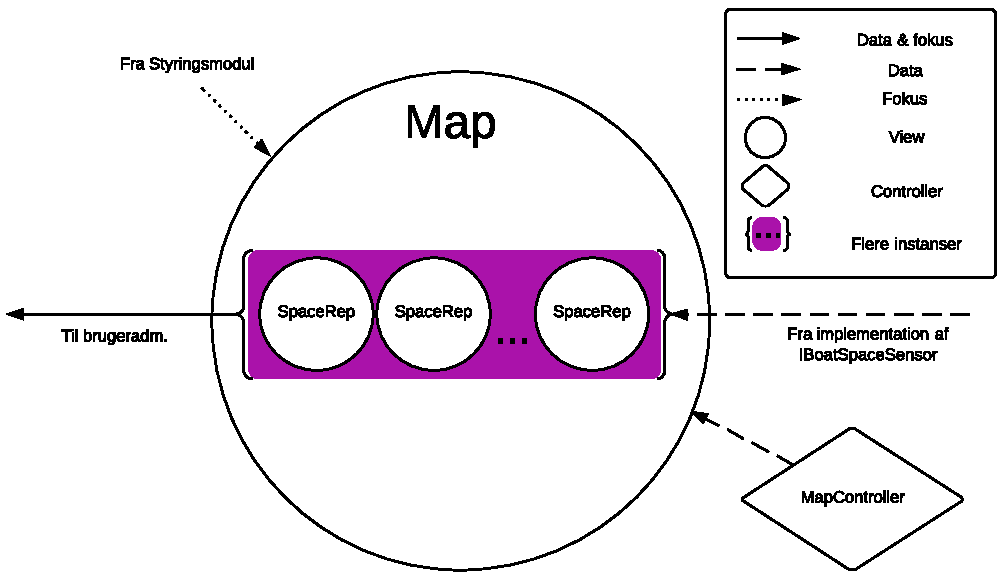
\includegraphics[width=\textwidth]{map-diagram.pdf}
  \caption{Oversigt over kort modulet.}
  \label{fig:map_diagram}
\end{figure}

Kortmodulet har til opgave at lave et kort, der giver et visuelt overblik over alle bådpladser der eksisterer på en havn.

\subsubsection{Funktionalitet}
\label{ssub:kort_funktionalitet}

Kortet præsenterer bådpladsers status i form af en beskrivende farve. Eksempelvis er en optaget bådplads status repræsenteret med farven rød, imens en fri bådplads status repræsenteres med farven grøn. Kortet skal modellere virkeligheden, således at virkelighedens informationer er reflekteret i kortet. Hvis et andet modul ændrer en bådplads status, skal dette modul skifte bådplads beskrivende farve til den tilsvarende. 


\subsubsection{Implementation}
\label{ssub:kort_implementation}

Det implementerede kort er opbygget af to lag. Et statisk baggrundslag, som viser havnens broer. Dertil et overliggende lag bestående af bådpladsrepræsentationer, der ligger i forhold til deres placering på baggrundslaget. En bådpladsrepræsentation er en reference til en bådplads i databasen. Når en bådplads i databasen ændrer status, ændres dennes repræsentation sig i takt.

Når der klikkes på en bådplads på kortet, kan følgende scenarier ske, afhængigt af hvilken bruger der klikker.

\begin{tabu} to \textwidth {XX}
  \toprule
  \textbf{Tilstand} & \textbf{Reaktion} \\
   \midrule
   Brugeren ligger selv ved bådpladsen & Brugeren bliver videresendt til et modul der viser oplysninger om brugeren \\
   \midrule
  Der ligger en anden bruger på bådpladsen, og brugeren har de nødvendige adgangstilladelser & Brugeren videresendes, til et modul der viser oplysninger om brugeren \\
  \midrule
   Brugeren er en gæst uden en eksisterende bådplads. Bådpladsen er ledig & Brugeren bliver sendt til et reservationsmodul \\ 
   \midrule
   Brugeren er en gæst med en eksisterende bådplads. Bådpladsen er ledig & Brugeren spørges om hvorvidt brugeren vil flytte til den nye plads \\
   \bottomrule 
\end{tabu}


Ved situationer der ikke matcher de ovenstående kriterier, sker der ingenting.


